\documentclass{article}
\usepackage[T1]{fontenc}
\usepackage{lmodern}
\usepackage{graphicx}
\usepackage{amsmath,amssymb}
\usepackage[a4paper,margin=2cm]{geometry}
\usepackage[absolute,overlay]{textpos}
\setlength{\TPHorizModule}{1mm}
\setlength{\TPVertModule}{1mm}
\usepackage[indonesian]{babel}
\usepackage{hyperref}
\setlength{\emergencystretch}{2em}
% unit: Halaman 16

\begin{document}

% === Halaman 16 (python/native) ===

• Contoh:  Bentuklah tabel perkalian untuk GF(11), kemudian tentukan solusi untuk 

x2   5 (mod 11)

Rinaldi Munir/II4021 Kriptografi

16

x2   5 (mod 11)

Maka:

   x2 = 16 → x1 = 4

   x2 = 49 → x2 = 7

 Cara lain:  cari elemen 

diagonal = 5, lalu ambil elemen

mendatar atau elemen 

Vertikalnya (dilingkari).

Sumber: Andreas Steffen, Elliptic Curve Cryptography

% deskripsi: gambar native xref 158
\noindent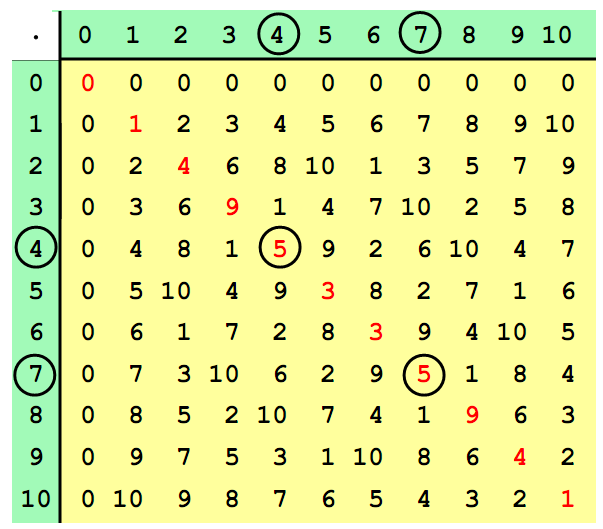
\includegraphics[width=0.85\textwidth]{../../images/python/page_016_img_01.png}

\end{document}
